%%%%%%%%%%%%%%%%%%%%%%%%%%%%%%%%%%%%%%%%%%%%%%%%%%%%%%%%%%%%%%%%%%%%%%%%%%%%%%%%
%2345678901234567890123456789012345678901234567890123456789012345678901234567890
%        1         2         3         4         5         6         7         8

%\documentclass[letterpaper, 10 pt, conference]{ieeeconf}  % Comment this line out if you need a4paper

\documentclass[a4paper, 10pt, conference]{ieeeconf}      % Use this line for a4 paper

\IEEEoverridecommandlockouts                              % This command is only needed if 
                                                          % you want to use the \thanks command

\overrideIEEEmargins                                      % Needed to meet printer requirements.

%In case you encounter the following error:
%Error 1010 The PDF file may be corrupt (unable to open PDF file) OR
%Error 1000 An error occurred while parsing a contents stream. Unable to analyze the PDF file.
%This is a known problem with pdfLaTeX conversion filter. The file cannot be opened with acrobat reader
%Please use one of the alternatives below to circumvent this error by uncommenting one or the other
%\pdfobjcompresslevel=0
%\pdfminorversion=4

% See the \addtolength command later in the file to balance the column lengths
% on the last page of the document

% The following packages can be found on http:\\www.ctan.org
%\usepackage{graphics} % for pdf, bitmapped graphics files
%\usepackage{epsfig} % for postscript graphics files
%\usepackage{mathptmx} % assumes new font selection scheme installed
%\usepackage{times} % assumes new font selection scheme installed
%\usepackage{amsmath} % assumes amsmath package installed
%\usepackage{amssymb}  % assumes amsmath package installed
\usepackage{textcomp}
\usepackage{hyperref}
\usepackage{amsmath,bm}
\usepackage{amssymb}
\usepackage{graphicx}
\usepackage{subcaption}
\usepackage{siunitx}
\usepackage{cite}
\usepackage{psfrag}
\usepackage{multirow}
\usepackage{flushend}

\title{\LARGE \bf
On the trochoidal motion model of a sensor\\placed off-centered inside a rolling ball
}

\author{Fabian Arzberger$^{1}$ and Andreas N{\"u}chter$^{1}$% <-this % stops a space
\thanks{$^{*}$We acknowledge funding from the ESA Contract No. 4000130925/20/NL/GLC for the study ``DAEDALUS -- Descent And Exploration in Deep Autonomy of Lava Underground Structures'' within the Open Space Innovation Platform (OSIP) lunar caves-system and the Elite Network Bavaria (ENB) for providing funds for the academic program ``Satellite Technology''}% <-this % stops a space
\thanks{$^{1}$The authors are with Computer Science XVII -- Robotics,
        Julius-Maximilians-Universit{\"a}t W{\"u}rzburg, 97074 Am Hubland, Germany.
        {Contact: \tt\small fabian.arzberger@uni-wuerzburg.de}}%
}


\begin{document}



\maketitle
\thispagestyle{empty}
\pagestyle{empty}


%%%%%%%%%%%%%%%%%%%%%%%%%%%%%%%%%%%%%%%%%%%%%%%%%%%%%%%%%%%%%%%%%%%%%%%%%%%%%%%%
\begin{abstract}
We study the motion model of a sensor rigidly mounted inside a ball, with the extrinsic parameters of the sensor with respect to the balls center of rotation being known by calibration.
Due to the rigid placement inside the ball, the geometry of the sensors trajectory resembles a 3D-Trochoid.
The motion model, which encorporates the angular velocities of the system, the radius of the ball, and the ground normal as input data, estimates the full 6-DoF pose of the sensor and is used in an extended Kalman-filter.
We deploy this motion model on our sherical mobile mapping platform to estimate the trajectory of a LiDAR sensor.
The evaluation shows that this approach improves the mapping accuracy, compared to our previous method which did not use a Kalman filter, and also compared to a more simple non-Trochoidal motion model using the Kalman-filter.     

\end{abstract}

\section{Introduction}
\section{Related work}

In the previous section, we have already introduced some spherical systems and their possible applications.
Our paper focuses on two major topics: 1) Extrinsic LiDAR calibration and 2) LiDAR-inertial odometry (LIO).
Note that the motion model presented in our paper only falls into the category of \textit{Inertial} odometry, yet we compare it with other LIO methods.
 
\subsection{Extrinsic LiDAR calibration}

Finding the extrinsic parameters between the coordinate systems of a LiDAR and some other sensor or reference frame is a broad, well studied field.
State-of-the-art approaches do not require the user to place artificial external markers in the environment but utilize the features or geometries of the environment directly.
The following methods are only a few examples that address the calibration of LiDAR-IMU systems.
In~\cite{Liu2020NovelMultifeature} the authors introduced an on-site calibration method for LiDAR-IMU systems that combines point, sphere, line, cylinder, and plane features.
Their approach employs a full information maximum likelihood estimation to obtain both the LiDAR-to-IMU extrinsics, but also the IMU intrinsic parameters.
Another similar approach that estimates both LiDAR-IMU extrinsic and IMU intrinsic parameters is~\cite{Liu2019ErrorModeling}, where the authors also utilize point, plane, cone, and cylinder features to construct a geometrically constrained optimization problem, followed by a restricted maximum likelihood estimation.
Li et al. present a method that employs ``continuous-time trajectory estimation wherein the IMU trajectory is modeled by Gaussian process regression with respect to the independent sampling timestamps''~\cite{Li2021CTTrajectory}.
Furthermore, they account for motion distortion effects of the LiDAR and match the corrected point clouds to a structured plane representation of the environment in an on-manifold batch-optimization framework.
In~\cite{Lv2022ObservabilityAware} the authors also utilize a continuous-time batch-optimization framework.
This approach has been designed for usage in degenerate cases by leveraging observability-aware modules, including an information-theoretic data selection policy and a state update mechanism that updates only the identifiable directions in the state space.
Note that in this work, it is specifically required to find the extrinsic translation parameters between the LiDAR and not the IMU, but rather the center point of rotation of the ball, which none of the abovementioned methods provide. 
These methods are still useful to find the extrinsic rotations.
However, as for translation, we have to introduce a new procedure specifically tailored for our use case.
Our approach is also marker-less and uses only the geometry of the environment via globally consistent scan-matching and utilizes the different radii that the sensor has when rotating around the center point.

\subsection{LiDAR-inertial odometry}

Many state-of-the-art approaches exist to solve the LIO problem, which is especially important for autonomous systems in GPS-denied environments.
Often, these methods have been developed and evaluated on cars~\cite{8967880}, UAV~\cite{s21123955}, or other rotationally more restricted systems when compared to a rolling ball. 
Currently, the most prominent approach to solving the LIO problem is to construct a tightly coupled optimization problem.
Some examples include~\cite{9760190}, where a factor graph is utilized to solve the optimization problem, or~\cite{9197567}, where the authors use an iterated error-state Kalman Filter.
Usually, state-of-the-art LIO methods also provide a motion distortion correction algorithm via IMU preintegration.
The most popular methods are open-source implementations like~\cite{huguet2022limo} for systems experiencing racing velocities, LIO-SAM~\cite{9341176} which utilizes local keyframes and also estimates the IMU bias errors, FAST-LIO~\cite{xu2022fast} which keeps a representation of the global map in an iteratively growing KD-tree, or DLIO~\cite{10160508} which provides a computationally efficient continuous-time coarse-to-fine approach.
In this work, we deploy two of the abovementioned state-of-the-art approaches on our spherical mobile mapping system, namely FAST-LIO in its most current version~\cite{xu2022fast}, and DLIO~\cite{10160508}.
In doing so we test if state-of-the-art methods are able to keep up with the faster than usual rotations and if these methods can reconstruct the trochoidal trajectory of the LiDAR.
We expect these methods to perform sub-optimally because the motion state propagation includes the accelerometer readings which, on rolling balls, are mostly governed by centripetal forces degrading their quality.     
\section{Extrinsic calibration}

\begin{figure}[h]
  \centering
  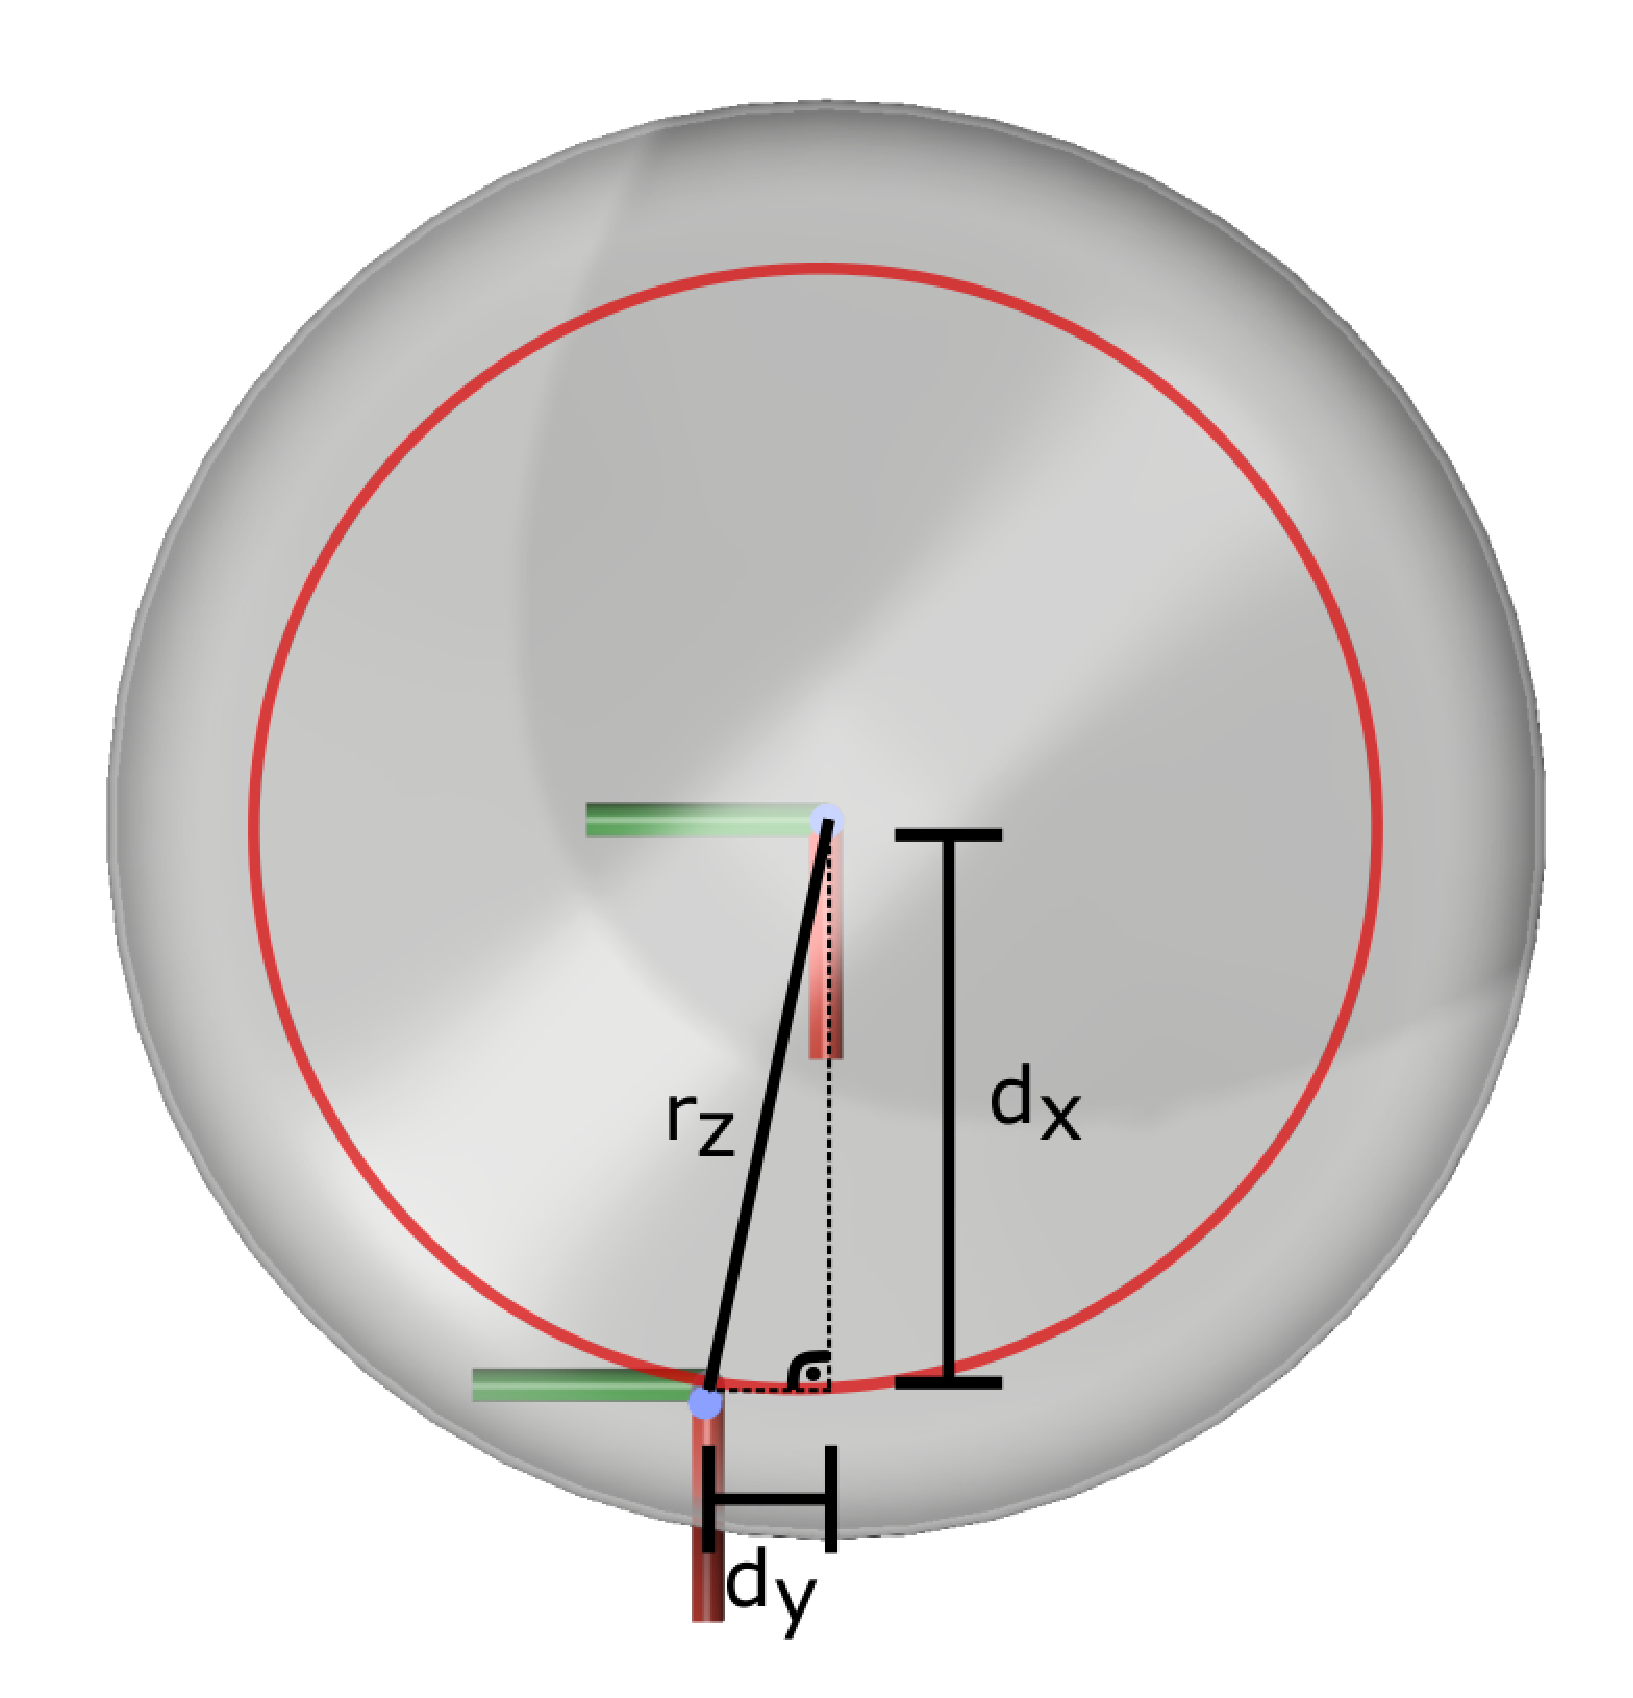
\includegraphics[width=.5\linewidth]{img/calibsphere}
  \caption{Calibration principle of a sensor inside a ball, illustrated in one axis.}
  \label{fig:calibsphere}
\end{figure}

The sensor, when mounted off-centered in the ball, will make circular trajectories if the ball rotates around an axis through its center.
We measure the radii of the sensor around the three orthogonal principal axes, which is enough information to construct the extrinsic parameters, describing the offset to the balls center.
\section{Trochoidal motion model}

\begin{figure*}
  \centering
  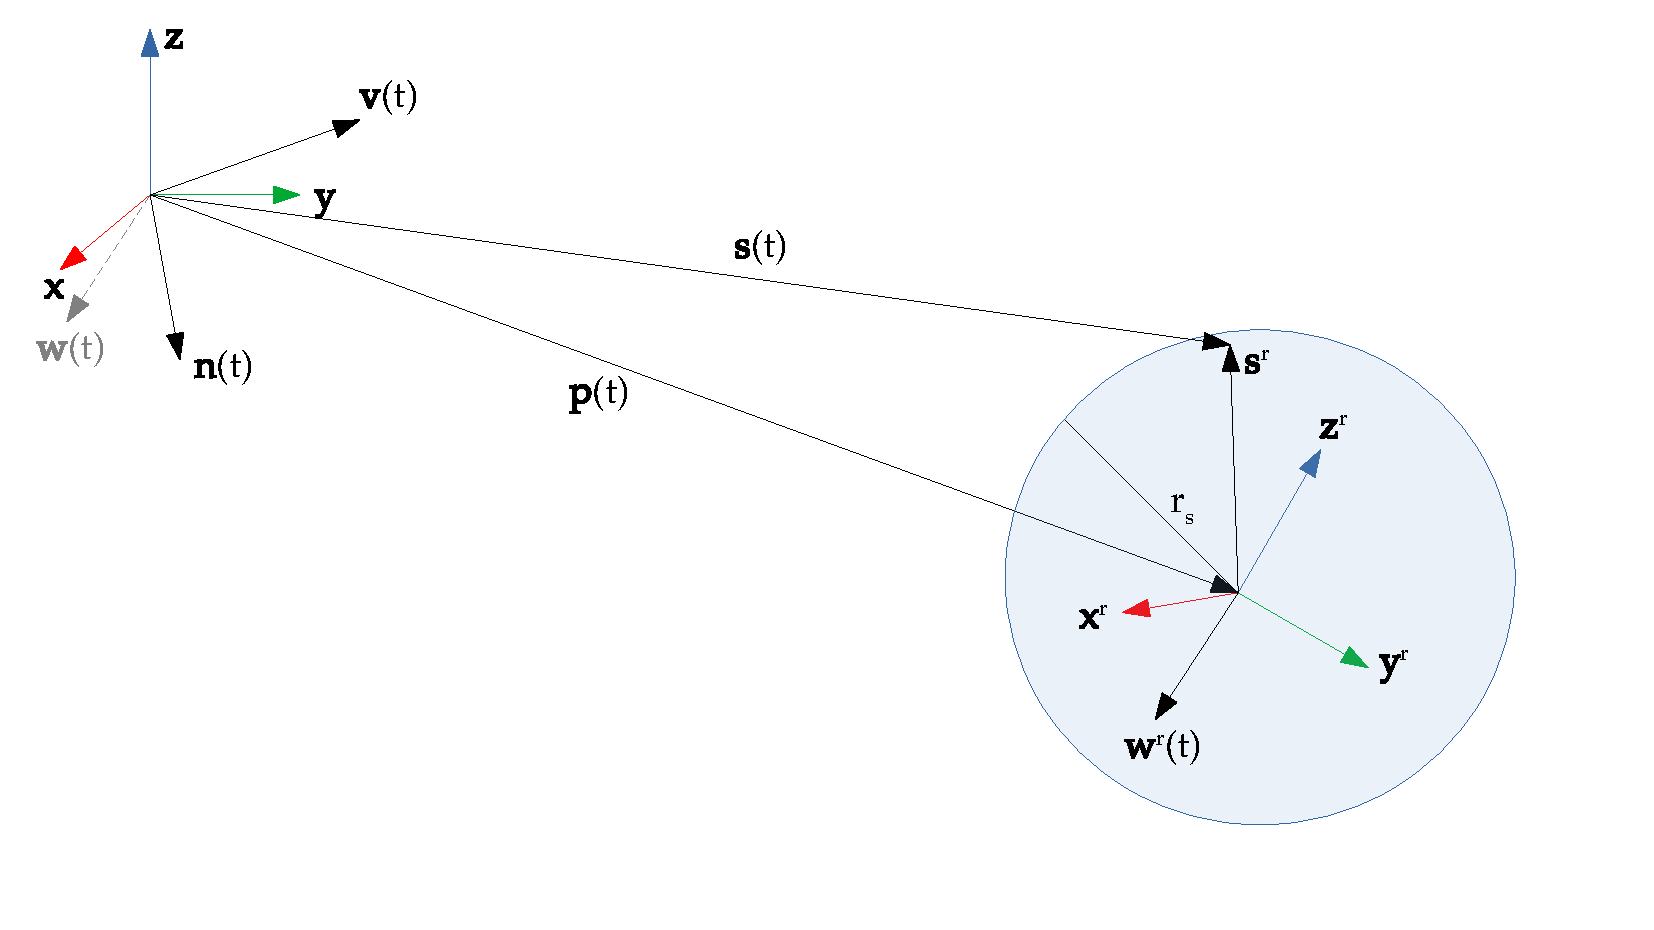
\includegraphics[width=.8\textwidth]{img/schematics}
  \caption{Schematics of the motion model}
  \label{fig:schematics}
\end{figure*}

The sensors rotation around the balls center is described through the rotation derivative which correspond to local gyro measurements $\vec{\omega}^r$   
\begin{align}
\frac{d}{dt}{\mathbf{R}}_r = \vec{\omega}^r_{\times} \cdot \mathbf{R}_r \;\; ,
\end{align}
where the cross-product matrix is defined as 
\begin{align}
\vec{\omega}_{\times} = 
\begin{pmatrix}
0 & -\omega_3 & \omega_2\\
\omega_3 & 0 & -\omega_1\\
-\omega_2 & \omega_1 & 0
\end{pmatrix} \;\; .
\end{align}
Go study group theory and learn about the Lie algebra $\mathfrak{so}(3)$ which is the tangent space to $\textrm{SO}(3)$ at its identity, to find out why this works. 
Anyways, through the inverse rotation we transform the local measurements into the global frame, leading to 
\begin{align}
\vec{\omega} = \mathbf{R}_r^{-1} \cdot \vec{\omega}^r
\end{align}
and
\begin{align}
\vec{s} = \mathbf{R}_r^{-1} \cdot \vec{s}^{\,r} + \,\vec{p}
\end{align}
with 
\begin{align}
\vec{p}(t) = \int_0^t \vec{v}(\tau) d\tau \;\; ,
\end{align}
where the velocity of the balls center over ground with normal $\vec{n}$ is
\begin{align}
\vec{v} = r_s \vec{\omega} \times \vec{n}\;\; .
\end{align}
The combined model:
\begin{align}
\vec{s} = \mathbf{R}_r^{-1} \cdot \vec{s}^{\,r} + \int \left( \left[ \mathbf{R}_r^{-1} \cdot r_s \cdot \vec{\omega}^r \right] \times \vec{n}\right)
\end{align}
expands, not ommiting the time dependence, to:
\begin{small}
  \begin{align}
    \vec{s}(t) &= \left[ \int_0^t \vec{\omega}^r_{\times}(\tau)\mathbf{R}_r(\tau)d\tau \right]^{-1} \vec{s}^{\,r} \\ \nonumber
    &+ \int_0^t\left( \left[ \bigg\{ \int_0^t \vec{\omega}^r_{\times}(\tau)\mathbf{R}_r(\tau)d\tau \bigg\} ^{-1} r_s \vec{\omega}^r(\tau) \right]\times \vec{n}(\tau) \right) d\tau
  \end{align}
\end{small}
which is the kinematic model to be solved numerically for any arbitrary gyro measurements.

\section{Extended Kalman filter}
\section{Implementation}
\section{Experimental evaluation}

\subsection{Trajectories}

\subsection{3D Point Clouds}

\section{Conclusions}

% \begin{appendix}

% \end{appendix}

% \section*{acknowledgment}

% \bibliographystyle{ieeetr}
% \bibliography{root}

\end{document}
